% Created by tikzDevice version 0.12 on 2019-07-24 04:41:22
% !TEX encoding = UTF-8 Unicode
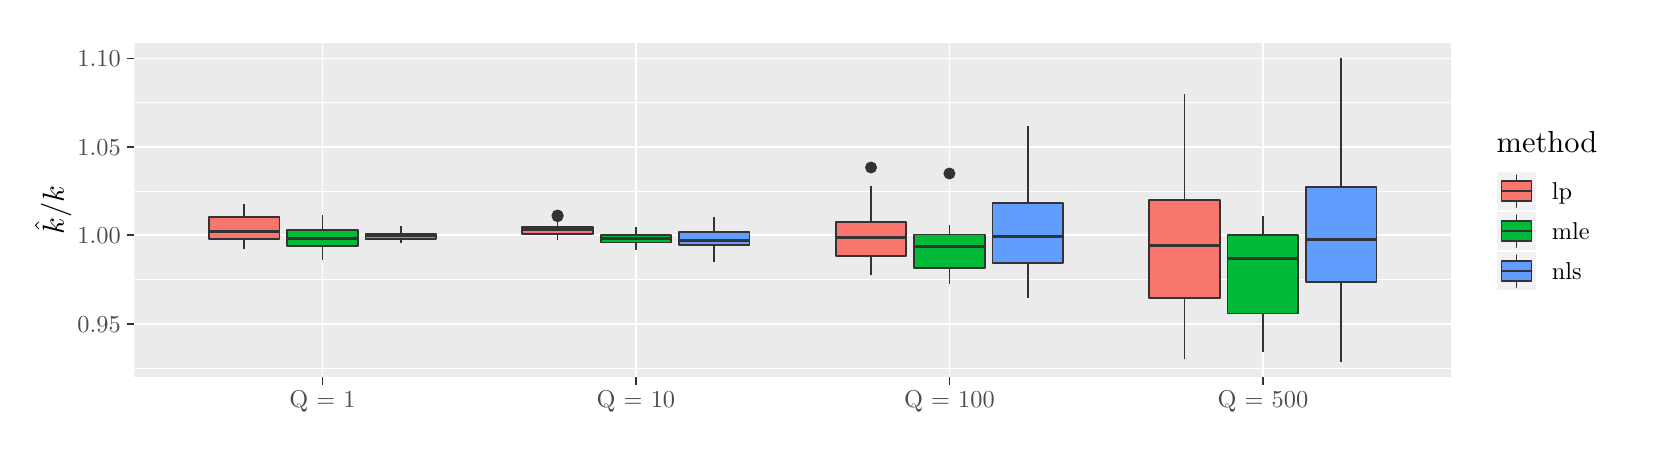
\begin{tikzpicture}[x=1pt,y=1pt]
\definecolor{fillColor}{RGB}{255,255,255}
\path[use as bounding box,fill=fillColor,fill opacity=0.00] (0,0) rectangle (578.16,144.54);
\begin{scope}
\path[clip] (  0.00,  0.00) rectangle (578.16,144.54);
\definecolor{drawColor}{RGB}{255,255,255}
\definecolor{fillColor}{RGB}{255,255,255}

\path[draw=drawColor,line width= 0.6pt,line join=round,line cap=round,fill=fillColor] (  0.00,  0.00) rectangle (578.16,144.54);
\end{scope}
\begin{scope}
\path[clip] ( 38.56, 18.22) rectangle (514.31,139.04);
\definecolor{fillColor}{gray}{0.92}

\path[fill=fillColor] ( 38.56, 18.22) rectangle (514.31,139.04);
\definecolor{drawColor}{RGB}{255,255,255}

\path[draw=drawColor,line width= 0.3pt,line join=round] ( 38.56, 21.58) --
	(514.31, 21.58);

\path[draw=drawColor,line width= 0.3pt,line join=round] ( 38.56, 53.54) --
	(514.31, 53.54);

\path[draw=drawColor,line width= 0.3pt,line join=round] ( 38.56, 85.50) --
	(514.31, 85.50);

\path[draw=drawColor,line width= 0.3pt,line join=round] ( 38.56,117.46) --
	(514.31,117.46);

\path[draw=drawColor,line width= 0.6pt,line join=round] ( 38.56, 37.56) --
	(514.31, 37.56);

\path[draw=drawColor,line width= 0.6pt,line join=round] ( 38.56, 69.52) --
	(514.31, 69.52);

\path[draw=drawColor,line width= 0.6pt,line join=round] ( 38.56,101.48) --
	(514.31,101.48);

\path[draw=drawColor,line width= 0.6pt,line join=round] ( 38.56,133.44) --
	(514.31,133.44);

\path[draw=drawColor,line width= 0.6pt,line join=round] (106.52, 18.22) --
	(106.52,139.04);

\path[draw=drawColor,line width= 0.6pt,line join=round] (219.79, 18.22) --
	(219.79,139.04);

\path[draw=drawColor,line width= 0.6pt,line join=round] (333.07, 18.22) --
	(333.07,139.04);

\path[draw=drawColor,line width= 0.6pt,line join=round] (446.34, 18.22) --
	(446.34,139.04);
\definecolor{drawColor}{gray}{0.20}

\path[draw=drawColor,line width= 0.6pt,line join=round] ( 78.20, 76.11) -- ( 78.20, 80.91);

\path[draw=drawColor,line width= 0.6pt,line join=round] ( 78.20, 68.28) -- ( 78.20, 64.52);
\definecolor{fillColor}{RGB}{248,118,109}

\path[draw=drawColor,line width= 0.6pt,line join=round,line cap=round,fill=fillColor] ( 65.46, 76.11) --
	( 65.46, 68.28) --
	( 90.94, 68.28) --
	( 90.94, 76.11) --
	( 65.46, 76.11) --
	cycle;

\path[draw=drawColor,line width= 1.1pt,line join=round] ( 65.46, 71.05) -- ( 90.94, 71.05);

\path[draw=drawColor,line width= 0.6pt,line join=round] (106.52, 71.31) -- (106.52, 76.77);

\path[draw=drawColor,line width= 0.6pt,line join=round] (106.52, 65.74) -- (106.52, 60.63);
\definecolor{fillColor}{RGB}{0,186,56}

\path[draw=drawColor,line width= 0.6pt,line join=round,line cap=round,fill=fillColor] ( 93.78, 71.31) --
	( 93.78, 65.74) --
	(119.26, 65.74) --
	(119.26, 71.31) --
	( 93.78, 71.31) --
	cycle;

\path[draw=drawColor,line width= 1.1pt,line join=round] ( 93.78, 68.29) -- (119.26, 68.29);

\path[draw=drawColor,line width= 0.6pt,line join=round] (134.84, 70.06) -- (134.84, 72.84);

\path[draw=drawColor,line width= 0.6pt,line join=round] (134.84, 68.07) -- (134.84, 66.65);
\definecolor{fillColor}{RGB}{97,156,255}

\path[draw=drawColor,line width= 0.6pt,line join=round,line cap=round,fill=fillColor] (122.09, 70.06) --
	(122.09, 68.07) --
	(147.58, 68.07) --
	(147.58, 70.06) --
	(122.09, 70.06) --
	cycle;

\path[draw=drawColor,line width= 1.1pt,line join=round] (122.09, 69.29) -- (147.58, 69.29);
\definecolor{fillColor}{gray}{0.20}

\path[draw=drawColor,line width= 0.4pt,line join=round,line cap=round,fill=fillColor] (191.48, 76.69) circle (  1.96);

\path[draw=drawColor,line width= 0.4pt,line join=round,line cap=round,fill=fillColor] (191.48, 76.41) circle (  1.96);

\path[draw=drawColor,line width= 0.6pt,line join=round] (191.48, 72.40) -- (191.48, 74.99);

\path[draw=drawColor,line width= 0.6pt,line join=round] (191.48, 70.09) -- (191.48, 67.86);
\definecolor{fillColor}{RGB}{248,118,109}

\path[draw=drawColor,line width= 0.6pt,line join=round,line cap=round,fill=fillColor] (178.73, 72.40) --
	(178.73, 70.09) --
	(204.22, 70.09) --
	(204.22, 72.40) --
	(178.73, 72.40) --
	cycle;

\path[draw=drawColor,line width= 1.1pt,line join=round] (178.73, 71.49) -- (204.22, 71.49);

\path[draw=drawColor,line width= 0.6pt,line join=round] (219.79, 69.71) -- (219.79, 72.69);

\path[draw=drawColor,line width= 0.6pt,line join=round] (219.79, 66.88) -- (219.79, 64.04);
\definecolor{fillColor}{RGB}{0,186,56}

\path[draw=drawColor,line width= 0.6pt,line join=round,line cap=round,fill=fillColor] (207.05, 69.71) --
	(207.05, 66.88) --
	(232.54, 66.88) --
	(232.54, 69.71) --
	(207.05, 69.71) --
	cycle;

\path[draw=drawColor,line width= 1.1pt,line join=round] (207.05, 68.40) -- (232.54, 68.40);

\path[draw=drawColor,line width= 0.6pt,line join=round] (248.11, 70.73) -- (248.11, 76.17);

\path[draw=drawColor,line width= 0.6pt,line join=round] (248.11, 65.97) -- (248.11, 59.73);
\definecolor{fillColor}{RGB}{97,156,255}

\path[draw=drawColor,line width= 0.6pt,line join=round,line cap=round,fill=fillColor] (235.37, 70.73) --
	(235.37, 65.97) --
	(260.86, 65.97) --
	(260.86, 70.73) --
	(235.37, 70.73) --
	cycle;

\path[draw=drawColor,line width= 1.1pt,line join=round] (235.37, 67.71) -- (260.86, 67.71);
\definecolor{fillColor}{gray}{0.20}

\path[draw=drawColor,line width= 0.4pt,line join=round,line cap=round,fill=fillColor] (304.75, 94.01) circle (  1.96);

\path[draw=drawColor,line width= 0.6pt,line join=round] (304.75, 74.28) -- (304.75, 87.22);

\path[draw=drawColor,line width= 0.6pt,line join=round] (304.75, 62.06) -- (304.75, 55.11);
\definecolor{fillColor}{RGB}{248,118,109}

\path[draw=drawColor,line width= 0.6pt,line join=round,line cap=round,fill=fillColor] (292.01, 74.28) --
	(292.01, 62.06) --
	(317.49, 62.06) --
	(317.49, 74.28) --
	(292.01, 74.28) --
	cycle;

\path[draw=drawColor,line width= 1.1pt,line join=round] (292.01, 68.55) -- (317.49, 68.55);
\definecolor{fillColor}{gray}{0.20}

\path[draw=drawColor,line width= 0.4pt,line join=round,line cap=round,fill=fillColor] (333.07, 91.84) circle (  1.96);

\path[draw=drawColor,line width= 0.6pt,line join=round] (333.07, 69.83) -- (333.07, 73.38);

\path[draw=drawColor,line width= 0.6pt,line join=round] (333.07, 57.67) -- (333.07, 51.78);
\definecolor{fillColor}{RGB}{0,186,56}

\path[draw=drawColor,line width= 0.6pt,line join=round,line cap=round,fill=fillColor] (320.33, 69.83) --
	(320.33, 57.67) --
	(345.81, 57.67) --
	(345.81, 69.83) --
	(320.33, 69.83) --
	cycle;

\path[draw=drawColor,line width= 1.1pt,line join=round] (320.33, 65.52) -- (345.81, 65.52);

\path[draw=drawColor,line width= 0.6pt,line join=round] (361.39, 81.23) -- (361.39,108.91);

\path[draw=drawColor,line width= 0.6pt,line join=round] (361.39, 59.62) -- (361.39, 46.82);
\definecolor{fillColor}{RGB}{97,156,255}

\path[draw=drawColor,line width= 0.6pt,line join=round,line cap=round,fill=fillColor] (348.64, 81.23) --
	(348.64, 59.62) --
	(374.13, 59.62) --
	(374.13, 81.23) --
	(348.64, 81.23) --
	cycle;

\path[draw=drawColor,line width= 1.1pt,line join=round] (348.64, 69.22) -- (374.13, 69.22);

\path[draw=drawColor,line width= 0.6pt,line join=round] (418.02, 82.31) -- (418.02,120.50);

\path[draw=drawColor,line width= 0.6pt,line join=round] (418.02, 46.87) -- (418.02, 24.87);
\definecolor{fillColor}{RGB}{248,118,109}

\path[draw=drawColor,line width= 0.6pt,line join=round,line cap=round,fill=fillColor] (405.28, 82.31) --
	(405.28, 46.87) --
	(430.77, 46.87) --
	(430.77, 82.31) --
	(405.28, 82.31) --
	cycle;

\path[draw=drawColor,line width= 1.1pt,line join=round] (405.28, 65.84) -- (430.77, 65.84);

\path[draw=drawColor,line width= 0.6pt,line join=round] (446.34, 69.69) -- (446.34, 76.44);

\path[draw=drawColor,line width= 0.6pt,line join=round] (446.34, 41.23) -- (446.34, 27.24);
\definecolor{fillColor}{RGB}{0,186,56}

\path[draw=drawColor,line width= 0.6pt,line join=round,line cap=round,fill=fillColor] (433.60, 69.69) --
	(433.60, 41.23) --
	(459.09, 41.23) --
	(459.09, 69.69) --
	(433.60, 69.69) --
	cycle;

\path[draw=drawColor,line width= 1.1pt,line join=round] (433.60, 61.26) -- (459.09, 61.26);

\path[draw=drawColor,line width= 0.6pt,line join=round] (474.66, 86.89) -- (474.66,133.55);

\path[draw=drawColor,line width= 0.6pt,line join=round] (474.66, 52.53) -- (474.66, 23.71);
\definecolor{fillColor}{RGB}{97,156,255}

\path[draw=drawColor,line width= 0.6pt,line join=round,line cap=round,fill=fillColor] (461.92, 86.89) --
	(461.92, 52.53) --
	(487.40, 52.53) --
	(487.40, 86.89) --
	(461.92, 86.89) --
	cycle;

\path[draw=drawColor,line width= 1.1pt,line join=round] (461.92, 67.85) -- (487.40, 67.85);
\end{scope}
\begin{scope}
\path[clip] (  0.00,  0.00) rectangle (578.16,144.54);
\definecolor{drawColor}{gray}{0.30}

\node[text=drawColor,anchor=base east,inner sep=0pt, outer sep=0pt, scale=  0.88] at ( 33.61, 34.53) {0.95};

\node[text=drawColor,anchor=base east,inner sep=0pt, outer sep=0pt, scale=  0.88] at ( 33.61, 66.49) {1.00};

\node[text=drawColor,anchor=base east,inner sep=0pt, outer sep=0pt, scale=  0.88] at ( 33.61, 98.45) {1.05};

\node[text=drawColor,anchor=base east,inner sep=0pt, outer sep=0pt, scale=  0.88] at ( 33.61,130.41) {1.10};
\end{scope}
\begin{scope}
\path[clip] (  0.00,  0.00) rectangle (578.16,144.54);
\definecolor{drawColor}{gray}{0.20}

\path[draw=drawColor,line width= 0.6pt,line join=round] ( 35.81, 37.56) --
	( 38.56, 37.56);

\path[draw=drawColor,line width= 0.6pt,line join=round] ( 35.81, 69.52) --
	( 38.56, 69.52);

\path[draw=drawColor,line width= 0.6pt,line join=round] ( 35.81,101.48) --
	( 38.56,101.48);

\path[draw=drawColor,line width= 0.6pt,line join=round] ( 35.81,133.44) --
	( 38.56,133.44);
\end{scope}
\begin{scope}
\path[clip] (  0.00,  0.00) rectangle (578.16,144.54);
\definecolor{drawColor}{gray}{0.20}

\path[draw=drawColor,line width= 0.6pt,line join=round] (106.52, 15.47) --
	(106.52, 18.22);

\path[draw=drawColor,line width= 0.6pt,line join=round] (219.79, 15.47) --
	(219.79, 18.22);

\path[draw=drawColor,line width= 0.6pt,line join=round] (333.07, 15.47) --
	(333.07, 18.22);

\path[draw=drawColor,line width= 0.6pt,line join=round] (446.34, 15.47) --
	(446.34, 18.22);
\end{scope}
\begin{scope}
\path[clip] (  0.00,  0.00) rectangle (578.16,144.54);
\definecolor{drawColor}{gray}{0.30}

\node[text=drawColor,anchor=base,inner sep=0pt, outer sep=0pt, scale=  0.88] at (106.52,  7.21) {Q = 1};

\node[text=drawColor,anchor=base,inner sep=0pt, outer sep=0pt, scale=  0.88] at (219.79,  7.21) {Q = 10};

\node[text=drawColor,anchor=base,inner sep=0pt, outer sep=0pt, scale=  0.88] at (333.07,  7.21) {Q = 100};

\node[text=drawColor,anchor=base,inner sep=0pt, outer sep=0pt, scale=  0.88] at (446.34,  7.21) {Q = 500};
\end{scope}
\begin{scope}
\path[clip] (  0.00,  0.00) rectangle (578.16,144.54);
\definecolor{drawColor}{RGB}{0,0,0}

\node[text=drawColor,rotate= 90.00,anchor=base,inner sep=0pt, outer sep=0pt, scale=  1.10] at ( 13.08, 78.63) {$\hat{k}/k$};
\end{scope}
\begin{scope}
\path[clip] (  0.00,  0.00) rectangle (578.16,144.54);
\definecolor{fillColor}{RGB}{255,255,255}

\path[fill=fillColor] (525.31, 43.84) rectangle (572.66,113.42);
\end{scope}
\begin{scope}
\path[clip] (  0.00,  0.00) rectangle (578.16,144.54);
\definecolor{drawColor}{RGB}{0,0,0}

\node[text=drawColor,anchor=base west,inner sep=0pt, outer sep=0pt, scale=  1.10] at (530.81, 99.27) {method};
\end{scope}
\begin{scope}
\path[clip] (  0.00,  0.00) rectangle (578.16,144.54);
\definecolor{drawColor}{RGB}{255,255,255}
\definecolor{fillColor}{gray}{0.95}

\path[draw=drawColor,line width= 0.6pt,line join=round,line cap=round,fill=fillColor] (530.81, 78.25) rectangle (545.26, 92.70);
\end{scope}
\begin{scope}
\path[clip] (  0.00,  0.00) rectangle (578.16,144.54);
\definecolor{drawColor}{gray}{0.20}

\path[draw=drawColor,line width= 0.6pt,line join=round,line cap=round] (538.03, 79.70) --
	(538.03, 81.86);

\path[draw=drawColor,line width= 0.6pt,line join=round,line cap=round] (538.03, 89.09) --
	(538.03, 91.26);
\definecolor{fillColor}{RGB}{248,118,109}

\path[draw=drawColor,line width= 0.6pt,line join=round,line cap=round,fill=fillColor] (532.61, 81.86) rectangle (543.45, 89.09);

\path[draw=drawColor,line width= 0.6pt,line join=round,line cap=round] (532.61, 85.48) --
	(543.45, 85.48);
\end{scope}
\begin{scope}
\path[clip] (  0.00,  0.00) rectangle (578.16,144.54);
\definecolor{drawColor}{RGB}{255,255,255}
\definecolor{fillColor}{gray}{0.95}

\path[draw=drawColor,line width= 0.6pt,line join=round,line cap=round,fill=fillColor] (530.81, 63.80) rectangle (545.26, 78.25);
\end{scope}
\begin{scope}
\path[clip] (  0.00,  0.00) rectangle (578.16,144.54);
\definecolor{drawColor}{gray}{0.20}

\path[draw=drawColor,line width= 0.6pt,line join=round,line cap=round] (538.03, 65.24) --
	(538.03, 67.41);

\path[draw=drawColor,line width= 0.6pt,line join=round,line cap=round] (538.03, 74.64) --
	(538.03, 76.81);
\definecolor{fillColor}{RGB}{0,186,56}

\path[draw=drawColor,line width= 0.6pt,line join=round,line cap=round,fill=fillColor] (532.61, 67.41) rectangle (543.45, 74.64);

\path[draw=drawColor,line width= 0.6pt,line join=round,line cap=round] (532.61, 71.02) --
	(543.45, 71.02);
\end{scope}
\begin{scope}
\path[clip] (  0.00,  0.00) rectangle (578.16,144.54);
\definecolor{drawColor}{RGB}{255,255,255}
\definecolor{fillColor}{gray}{0.95}

\path[draw=drawColor,line width= 0.6pt,line join=round,line cap=round,fill=fillColor] (530.81, 49.34) rectangle (545.26, 63.80);
\end{scope}
\begin{scope}
\path[clip] (  0.00,  0.00) rectangle (578.16,144.54);
\definecolor{drawColor}{gray}{0.20}

\path[draw=drawColor,line width= 0.6pt,line join=round,line cap=round] (538.03, 50.79) --
	(538.03, 52.96);

\path[draw=drawColor,line width= 0.6pt,line join=round,line cap=round] (538.03, 60.18) --
	(538.03, 62.35);
\definecolor{fillColor}{RGB}{97,156,255}

\path[draw=drawColor,line width= 0.6pt,line join=round,line cap=round,fill=fillColor] (532.61, 52.96) rectangle (543.45, 60.18);

\path[draw=drawColor,line width= 0.6pt,line join=round,line cap=round] (532.61, 56.57) --
	(543.45, 56.57);
\end{scope}
\begin{scope}
\path[clip] (  0.00,  0.00) rectangle (578.16,144.54);
\definecolor{drawColor}{RGB}{0,0,0}

\node[text=drawColor,anchor=base west,inner sep=0pt, outer sep=0pt, scale=  0.88] at (550.76, 82.45) {lp};
\end{scope}
\begin{scope}
\path[clip] (  0.00,  0.00) rectangle (578.16,144.54);
\definecolor{drawColor}{RGB}{0,0,0}

\node[text=drawColor,anchor=base west,inner sep=0pt, outer sep=0pt, scale=  0.88] at (550.76, 67.99) {mle};
\end{scope}
\begin{scope}
\path[clip] (  0.00,  0.00) rectangle (578.16,144.54);
\definecolor{drawColor}{RGB}{0,0,0}

\node[text=drawColor,anchor=base west,inner sep=0pt, outer sep=0pt, scale=  0.88] at (550.76, 53.54) {nls};
\end{scope}
\end{tikzpicture}
